\documentclass[thesis.tex]{subfiles}

\begin{document}

Now with the ability to calculate open-shell states, properties of and transitions between these states can be obtained.  In particular, this chapter focuses on beta-decay transitions between two particle-attached states and between two particle-removed states.  However, because these techniques are formulated in a general way, they can be applied to any type of one-body operator and any type of EOM-CC state.  First, this chapter describes beta-decay processes in detail and the relevant operators are introduced.  Then, these operators are used to construct effective coupled cluster operators that take important correlations from the ground-state wave function into account.  Finally, the effective operators are applied to EOM-CC states to calculate transition amplitudes for the corresponding processes.  These amplitudes can then be used to calculate observables like decay strengths and half-lives.

\section{Beta-Decay Properties} \label{section:betaproperties}

Nuclear beta decay describes a class of radioactive decays of the atomic nucleus that result as a consequence of the weak interaction.  These processes involve the exchange of a $\mathrm{W}$ boson which allows a quark within a proton or neutron to change type, thus converting a neutron to a proton or vice versa.  Additionally, this conversion is accompanied by an electron-antineutrino or positron-neutrino pair which ensures the process conserves charge and lepton number.  This work focuses on the three most common types of weak processes that occur within atomic nuclei: $\beta^{-}$ decay, $\beta^{+}$ decay, and electron capture (EC).  The first, $\beta^{-}$ decay, is the process whereby a down quark becomes an up quark, converting a neutron to a proton along with the creation of an electron, or $\beta^{-}$ particle, and an antineutrino.  Schematically, this decay can be written as,
\begin{equation*}
  \beta^{-}\ \text{decay}:  \hspace{0.5cm}  n\ &\longrightarrow\ p + e^{-} + \bar{\nu}_{e}.
\end{equation}
The corresponding mirror process is the $\beta^{+}$ decay, whereby an up quark becomes a down quark, converting a proton to a neutron with the creation of a positron, or $\beta^{+}$ particle, and a neutrino.  This decay is represented by,
\begin{equation*}
  \beta^{+}\ \text{decay}:  \hspace{0.5cm}   p\ &\longrightarrow\ n + e^{+} + \nu_{e}.
\end{equation}
A closely related process is the electron capture, whereby an atomic electron interacts with an up quark of a proton via a $\mathrm{W}$ boson, causing the conversion to a down quark and the release of a neutrino.  This process can be written as,
\begin{equation*}
  \text{Electron capture}:  \hspace{0.5cm}   p + e^{-}\ &\longrightarrow\ n + \nu_{e}.
\end{equation}
These three processes are schematically represented in Fig.\ \ref{fig:beta-0}.

\begin{figure}[h]
  \centering
  \begin{subfigure}{0.3333\linewidth}
    \centering
    \hspace{0.1cm}
    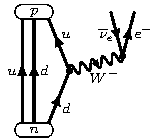
\includegraphics[height=3.5cm]{betadecay/BetaDecay-figure0.pdf}
    \caption{}
    \label{fig:beta-minus-0}
  \end{subfigure}
  \hspace{-0.05\linewidth}
  \begin{subfigure}{0.3333\linewidth}
    \centering
    \hspace{0.1cm}
    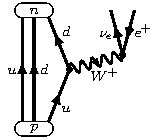
\includegraphics[height=3.5cm]{betadecay/BetaDecay-figure1.pdf}
    \caption{}
    \label{fig:beta-plus-0}
  \end{subfigure}
  \hspace{-0.05\linewidth}
  \begin{subfigure}{0.3333\linewidth}
    \centering
    \hspace{0.1cm}
    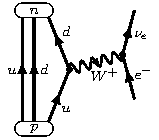
\includegraphics[height=3.5cm]{betadecay/BetaDecay-figure2.pdf}
    \caption{}
    \label{fig:beta-ec-0}
  \end{subfigure}
  \caption{Schematic representations of the three free-space weak processes in this work: $\beta^{-}$ decay (a), $\beta^{+}$ decay (b), and electron-capture (c).  The coupling constant for the point interaction vertex is the weak-interaction coupling constant $g_{W}$.}
  \label{fig:beta-0}
\end{figure}


The decay $Q$-value is a measure of the net energy of these processes.  In free space, only $\beta^{-}$ decay has a positive $Q$-value and can occur spontaneously.  However, within a nucleus, correlations between nucleons cause the relatively-simple exchanges in Fig.\ \ref{fig:beta-0} to take on more complicated, higher-order processes involving pion exchanges between different nucleons, see Fig.\ \ref{fig:beta-2}.  This also has the effect of changing the energetics of the $\beta^{+}$ decay and electron-capture processes such that their Q-values are positive and can occur within certain nuclei.  However, these complicated processes can be approximated by assuming that the weak interaction occurs at very short length and time scales  due to the large mass of the $\mathrm{W}$ boson, $m_{W}$.  Known as the \textit{impulse approximation}, this treatment of beta-decay reduces the many-body processes involves one nucleon as a spectator to the other nucleons, shown in Fig.\ \ref{fig:beta-1}.  In addition, this motivates the simplification of the $\mathrm{W}$ boson exchanges in Fig.\ \ref{fig:beta-0}, with coupling constant $g_{W}$, to a point interaction, shown in Figs.\ \ref{fig:beta-1} and \ref{fig:beta-2}, with an effective coupling constant $G_{F} = \sqrt{2}g_{W}^{2}/8(m_{W}c^{2})^{2}$ \cite{HALZEN1984}.

\begin{figure}
  \centering
  \begin{subfigure}{0.3333\linewidth}
    \centering
    \hspace{0.1cm}
    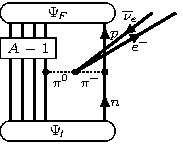
\includegraphics[height=3.5cm]{betadecay/BetaDecay-figure6.pdf}
    \caption{}
    \label{fig:beta-minus-2}
  \end{subfigure}
  \hspace{-0.05\linewidth}
  \begin{subfigure}{0.3333\linewidth}
    \centering
    \hspace{0.1cm}
    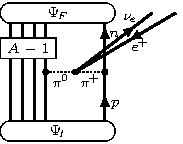
\includegraphics[height=3.5cm]{betadecay/BetaDecay-figure7.pdf}
    \caption{}
    \label{fig:beta-plus-2}
  \end{subfigure}
  \hspace{-0.05\linewidth}
  \begin{subfigure}{0.3333\linewidth}
    \centering
    \hspace{0.1cm}
    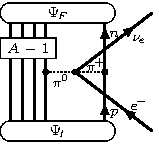
\includegraphics[height=3.5cm]{betadecay/BetaDecay-figure8.pdf}
    \caption{}
    \label{fig:beta-ec-2}
  \end{subfigure}
  \caption{Schematic representations of a higher-order weak interactions involving pion-exchange that occur within a nucleus, for $\beta^{-}$ decay (a), $\beta^{+}$ decay (b), and electron-capture (c).  These processes are not included in the impulse approximation.    The coupling constant for the point interaction vertex is the effective weak-interaction coupling constant $G_{F}$.}
  \label{fig:beta-2}
\end{figure}

\begin{figure}
  \centering
  \begin{subfigure}{0.3333\linewidth}
    \centering
    \hspace{0.1cm}
    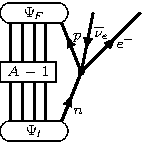
\includegraphics[height=3.5cm]{betadecay/BetaDecay-figure3.pdf}
    \caption{}
    \label{fig:beta-minus-1}
  \end{subfigure}
  \hspace{-0.05\linewidth}
  \begin{subfigure}{0.3333\linewidth}
    \centering
    \hspace{0.1cm}
    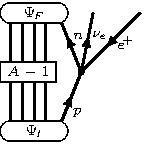
\includegraphics[height=3.5cm]{betadecay/BetaDecay-figure4.pdf}
    \caption{}
    \label{fig:beta-plus-1}
  \end{subfigure}
  \hspace{-0.05\linewidth}
  \begin{subfigure}{0.3333\linewidth}
    \centering
    \hspace{0.1cm}
    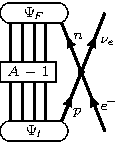
\includegraphics[height=3.5cm]{betadecay/BetaDecay-figure5.pdf}
    \caption{}
    \label{fig:beta-ec-1}
  \end{subfigure}
  \caption{Schematic representations of the impulse approximations to the different weak processes within an $A$-body nucleus: $\beta^{-}$ decay (a), $\beta^{+}$ decay (b), and electron-capture (c).  The active nucleon doesn't interact with the initial and final nuclei during the weak process.  The coupling constant for each interation vertex is the weak-interaction coupling constant $G_{F}$.}
  \label{fig:beta-1}
\end{figure}

These beta-decay processes can be further characterized by the character of their angular momentum.  \textit{Allowed} beta decays involve an electron-antineutrino or positron-neutrino pair with no angular momentum, $L=0$.  In this case, there can be no parity change between the initial and final nuclear states.  Also, each pair of spin-$\frac{1}{2}$ leptons carries a coupled spin of either $S=0$ or $S=1$.  Therefore, the initial and final nuclear states must have angular momenta that only differ by $0$ or $1$, ($\Delta J = 0, 1$).  Additionally, parity must be conserved for these interactions.  \textit{Fermi transitions} (F) occur when the nuclear states are coupled to leptons with $S=0$, and \textit{Gamow-Teller transitions} (GT) occur when the the lepton have a spin $S=1$.  The summary of these selection rules are shown in table\ \ref{tab:beta-selection}.
\begin{table}[h]
  \centering
  \begin{tabular}{ l @{\hskip 50pt} l @{\hskip 50pt} l } \hline
    \vspace{0.1mm} \\
    Decay Type     & $\Delta J = J_{F} - J_{I}$ & $\pi_{F}\pi_{I}$ \vspace{0.5mm} \\ \hline\hline
    \vspace{0.5mm} \\
    Fermi          & 0                         & +1 \\
    Gamow-Teller   & $1    (J_{F}=0\ \text{or}\ J_{I}=0)$   & +1 \\
    Gamow-Teller   & $0,1  (J_{F}>0\ \text{and}\ J_{I}>0)$  & +1 \vspace{1mm} \\ \hline
  \end{tabular}
  \caption{Summary of the selection rules for allowed beta decays according to the angular momentum $J$ and parity $\pi$ of the initial ($I$) and final ($F$) states.}
  \label{tab:beta-selection}
\end{table}

The half-life of these processes $T_{1/2}$ can be calculated using a combination of both the Fermi and Gamow-Teller type transitions in the form of their reduced transition amplitudes, $B_{\text{F}}$ and $B_{\text{GT}}$, respectively,
\begin{equation} \label{eq:RTAmps}
  B_{F} = \frac{g_{V}^{2} \lvert M_{F} \rvert^{2}}{2J_{i} + 1} \hspace{0.75cm} B_{GT} = \frac{g_{A}^{2} \lvert M_{GT} \rvert^{2}}{2J_{i} + 1},
\end{equation}
where $J_{i}$ is the final state angular momentum.  The factor $g_{V}$ is the vector coupling constant, and its value is can be shown to be exactly $g_{V}=1.0$.  The axial-vector coupling constant $g_{A}$ has a free-space value of $g_{A}=-g_{V}$, but is altered within nuclei due to nucleon-nucleon correlations.  The exact problem of how to treat the value of the axial-vector constant has been a widely studied topic for decades \cite{HARDY2005,TOWNER2008,KUBODERA1978,OSET1979}, but this work will use the value $g_{A}/g_{V} = 1.261(8)$ \cite{WILKINSON1982474}.  The transition matrix elements $M_{F}$ and $M_{GT}$ are measures of the overlap integral between the initial and final nuclear states for the different transitions and will be discussed in the next section.  Inserting these reduced transition amplitudes into the standard result from time-dependent perturbation theory gives the decay half-life,
\begin{equation}
  T_{1/2} = \frac{f}{K_{0}\left( B_{\text{F}} + B_{\text{GT}} \right)}.
\end{equation}
The factor $f$ represents a phase-space integral over the final nuclear and lepton states and depends on the decay Q-value. The factor $K_{0}$ encodes the relevant constants involved,
\begin{equation}
  K_{0} = \frac{2\pi^{3}\hbar^{7}\ln 2}{m_{e}^{5}c^{4}G_{F}^{2}} \approx 6147 sec,
\end{equation}
where $m_{e}$ is the electron mass, and $G_{F}$ is the effective coupling constant.  The next section describes the process of improving upon the impulse approximation by using coupled cluster theory to include higher-body interactions with the CC similarity transformation.


\section{Coupled Cluster Effective Operators} \label{section:cc-operators}

The main step in calculating dynamic properties within an \emph{ab initio} framework is to calculate the transition matrix elements of the relevant operator between two correlated many-body states.  In the cases considered in this thesis, the correlated many-body states are given by right and left expansions for the PA-EOM(2) and PR-EOM(2) operators in Eqs.\ \eqref{eq:pa-eom2} and \eqref{eq:pr-eom2}, respectively.  Beta-decay properties are computed with the Fermi and Gamow-Teller operators which are one-body operators that change a neutron to a proton or vice versa and carry the quantum numbers that correspond to the rules in table \ref{tab:beta-selection}.

In the impulse approximation, the Fermi operator, which has no spin component, is simply equivalent to the isospin raising operator for the $\beta^{-}$ Fermi transition, which changes a neutron to a proton, or the lowering operator for the $\beta^{+}$ transition, which changes a proton to a neutron,
\begin{equation}
  \Oop{}_{F^{\mp}} = \sum_{pq}\relement{p}{\mathbf{\hat{\tau}_{\pm}}}{q} \normord{\co{p}\ao{q}}.
\end{equation}
The reduced matrix element, see appendix \ref{chapter:angular_momentum}, $\relement{p}{\mathbf{\hat{\tau}_{\pm}}}{q}$, is given for harmonic-oscillator basis states \cite{SUHONEN2007},
\begin{equation}
  \relement{p}{\mathbf{\hat{\tau}_{\pm}}}{q} = \sqrt{2j_{p} + 1}\ \delta_{n_{p}n_{q}}\delta_{l_{p}l_{q}}\delta_{j_{p}j_{q}}\delta_{t_{p}t_{q}\pm 1}\ .
\end{equation}
Similarly, the Gamow-Teller operator also includes the isospin raising/lowering operator in addition to the spin operator $\hat{\sigma}$,
\begin{equation}
  \Oop{}_{GT^{\mp}} = \sum_{pq}\relement{p}{\mathbf{\hat{\sigma}\hat{\tau}_{\pm}}}{q} \normord{\co{p}\ao{q}}.
\end{equation}
Here, the reduced matrix element, $\relement{p}{\mathbf{\hat{\sigma}\hat{\tau}_{\pm}}}{q}$, is also given for the harmonic-oscillator basis \cite{SUHONEN2007},
\begin{equation}
  \relement{p}{\mathbf{\hat{\sigma}\hat{\tau}_{\pm}}}{q} = \sqrt{6(2j_{p} + 1)(2j_{q} + 1)}\sixj{\frac{1}{2}}{\frac{1}{2}}{1}{j_{q}}{j_{p}}{l_{p}} \mathop{(-1)^{l_{p}+j_{p}+\frac{3}{2}}} \delta_{n_{p}n_{q}}\delta_{l_{p}l_{q}}\delta_{t_{p}t_{q}\pm 1}.
\end{equation}

These operators can now be used to calculate the transition matrix elements in Eq.\ \eqref{eq:RTAmps} by applying them between an initial state, $\ket{\Corr_{\mathrm{i}}}$, and a final state, $\bra{\Corr_{\mathrm{f}}}$.  The Fermi reduced transition amplitude is,
\begin{equation} \label{eq:fermi-ME}
  M_{F} = \relement{\Corr_{\mathrm{f}}}{\Oop{}_{F^{\mp}}}{\Corr_{\mathrm{i}}} = \delta_{J_\mathrm{f}J_{\mathrm{i}}}\sum_{pq}\relement{p}{\mathbf{\hat{\tau}_{\pm}}}{q}\relement{\Corr_{\mathrm{f}}}{\normord{\co{p}\ao{q}}}{\Corr_{\mathrm{i}}}.
\end{equation}
Similarly, the Gamow-Teller reduced transition amplitude is,
\begin{equation} \label{eq:gamowteller-ME}
  M_{GT} = \relement{\Corr_{\mathrm{f}}}{\Oop{}_{GT^{\mp}}}{\Corr_{\mathrm{i}}} = \sum_{pq}\relement{p}{\mathbf{\hat{\sigma}\hat{\tau}_{\pm}}}{q}\relement{\Corr_{\mathrm{f}}}{\normord{\co{p}\ao{q}}}{\Corr_{\mathrm{i}}}.
\end{equation}

Within the coupled cluster framework, the initial and final states take the form of PA-EOM or PR-EOM states given generically in Eq.\ \eqref{eq:eom_def}.  According to Eqs.\ \eqref{eq:eom_schrodinger1} and \eqref{eq:eom_dual1}, the left and right eigenstates of the bare Hamiltonian can be given by $\bra{\Corr_{\mathrm{f}}} = \refbra\Lop_{\mathrm{f}}\E^{-\Top}$ and $\ket{\Corr_{\mathrm{i}}} = \E^{\Top}\Rop_{\mathrm{i}}\refket$.  Inserting these EOM states into Eqs.\ \eqref{eq:fermi-ME} and \eqref{eq:gamowteller-ME}, gives,
\begin{equation} \label{eq:fermi-ME-EOM}
  M_{F} = \delta_{J_\mathrm{f}J_{\mathrm{i}}}\sum_{pq}\relement{p}{\mathbf{\hat{\tau}_{\pm}}}{q}\relement{\Ref}{\Lop_{\mathrm{f}}\E^{-\Top}\normord{\co{p}\ao{q}}\E^{\Top}\Rop_{\mathrm{i}}}{\Ref}.
\end{equation}
Similarly, the Gamow-Teller matrix element becomes,
\begin{equation} \label{eq:gamowteller-ME-EOM}
  M_{GT} = \sum_{pq}\relement{p}{\mathbf{\hat{\sigma}\hat{\tau}_{\pm}}}{q}\relement{\Ref}{\Lop_{\mathrm{f}}\E^{-\Top}\normord{\co{p}\ao{q}}\E^{\Top}\Rop_{\mathrm{i}}}{\Ref}.
\end{equation}

The resemblance of these equations to to Eq.\ \eqref{eq:cc_heff0} motivates the construction of an \texit{effective operator}, $\EOop{\lambda}$.  The Fermi and Gamow-Teller effective operators have the form,
\begin{gather}
  \EOop{}_{F^{\mp}} = \sum_{pq}\relement{p}{\mathbf{\hat{\tau}_{\pm}}}{q} \E^{-\Top}\normord{\co{p}\ao{q}}\E^{\Top}, \\
  \EOop{}_{GT^{\mp}} = \sum_{pq}\relement{p}{\mathbf{\hat{\sigma}\hat{\tau}_{\pm}}}{q} \E^{-\Top}\normord{\co{p}\ao{q}}\E^{\Top}.
\end{gather}
The similarity-transformed component, $\E^{-\Top}\normord{\co{p}\ao{q}}\E^{\Top}$, is known as the \textit{one-body density matrix}.  Using the Baker-Campbell-Housedorf expansion like Eq.\ \eqref{eq:bch-cc} and the reduction to connected diagrams like Eq.\ \eqref{eq:cc_heff1}, the one-body density matrix can be reduced to the form,
\begin{equation} \label{eq:eff_OBD}
  \E^{-\Top}\normord{\co{p}\ao{q}}\E^{\Top} = \left(\normord{\co{p}\ao{q}} e^{\Top}\right)_{\mathrm{c}}.
\end{equation}
The effective operators are best calculated using diagrammatic techniques like those used for the effective Hamiltonian.  In this case, the bare one-body operators are depicted by the vertex type \raisebox{-5pt}{\mbox{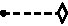
\includegraphics[height=17pt]{diagrams/Eff_1b/Eff_1b-figure13.pdf}}} while the effective one- and two-body operators are depicted by \raisebox{-5pt}{\mbox{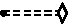
\includegraphics[height=17pt]{diagrams/Eff_1b/Eff_1b-figure14.pdf}}} and \raisebox{-5pt}{\mbox{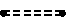
\includegraphics[height=17pt]{diagrams/Eff_1b/Eff_1b-figure15.pdf}}}, respectively.

The one-body beta-decay operators can be split into $\mathrm{hp}$, $\mathrm{hh}$, $\mathrm{pp}$, and $\mathrm{ph}$ components which are analogous to the one-body components of the effective Hamiltonian, see \ref{chapter:eff_ham_diagrams}.  The $\mathrm{hp}$ component has no connected terms in Eq.\ \eqref{eq:eff_OBD}, and so it is unchanged by the similarity transformation,
\begin{align}
  \diagram{Eff_1b/Eff_1b-figure0} &= \diagram{Eff_1b/Eff_1b-figure1} \notag \\
  \oopint{\lambda}{i}{a} &= \opint{\lambda}{i}{a}.
\end{align}
The $\mathrm{pp}$ component is augmented by single excitations from the reference state.  This component's diagrammatic and algebraic expressions are,
\begin{align}
  \diagram{Eff_1b/Eff_1b-figure2} &= \diagram{Eff_1b/Eff_1b-figure3} + \diagram{Eff_1b/Eff_1b-figure4} \notag \\
  \oopint{\lambda}{a}{b} &= \opint{\lambda}{a}{b} - \sum\limits_{k}\oopint{\lambda}{k}{b}\tamp{a}{k}.
\end{align}
Similarly, the $\mathrm{hh}$ component is also augmented by single excitations from the reference state,
\begin{align}
  \diagram{Eff_1b/Eff_1b-figure5} &= \diagram{Eff_1b/Eff_1b-figure6} + \diagram{Eff_1b/Eff_1b-figure7} \notag \\
  \oopint{\lambda}{i}{j} &= \opint{\lambda}{i}{j} + \sum\limits_{c}\oopint{\lambda}{i}{c}\tamp{c}{j}.
\end{align}
The $\mathrm{ph}$ component of the effective beta-decay operator includes effects from single and double excitations from the reference state.  The diagrammatic and algebraic expressions for this component are,
\begin{align}
  \diagram{Eff_1b/Eff_1b-figure8} &= \diagram{Eff_1b/Eff_1b-figure9} + \diagram{Eff_1b/Eff_1b-figure10} + \diagram{Eff_1b/Eff_1b-figure11} + \diagram{Eff_1b/Eff_1b-figure12} \notag \\
  \oopint{\lambda}{a}{i} &= \opint{\lambda}{a}{i} + \sum\limits_{\mathclap{c}}\oopint{\lambda}{a}{c}\tamp{c}{i} - \sum\limits_{\mathclap{k}}\oopint{\lambda}{k}{i}\tamp{a}{k} + \sum\limits_{\mathclap{kc}}\oopint{\lambda}{k}{c}\tamp{ac}{ik}.
\end{align}

Like the higher-body interactions induced by the CC similarity transformation, two-body effective operators are induced from the one-body bare beta-decay operator.  Calculating properties using PA-EOM(2) and PR-EOM(2) states requires only two components of the effective two-body operator.  The $\mathrm{pphp}$ component is the results of double excitations from the reference state and is given by the following diagram and the corresponding expression,
\begin{align}
  \diagram{Eff_2b/Eff_2b-figure0} &= \diagram{Eff_2b/Eff_2b-figure1} \notag \\
  \oopint{\lambda}{ab}{ic} &= -\sum\limits_{k}\oopint{\lambda}{k}{c}\tamp{ab}{ik}.
\end{align}
Similarly, the $\mathrm{hphh}$ component is represented by the following diagram and its corresponding algebraic expression,
\begin{align}
  \diagram{Eff_2b/Eff_2b-figure2} &= \diagram{Eff_2b/Eff_2b-figure3} \notag \\
  \oopint{\lambda}{ia}{jk} &= \sum\limits_{c}\oopint{\lambda}{i}{c}\tamp{ca}{jk}.
\end{align}

To see how the matrix elements change as they are transformed, the difference between selected bare Gamow-Teller matrix elements $\relement{p}{\mathbf{\hat{\sigma}\hat{\tau}_{\pm}}}{q}$ and the similarity tranformed quantities are shown in Fig. \ref{fig:GTMEs}.
\begin{figure}[h]
  \centering
  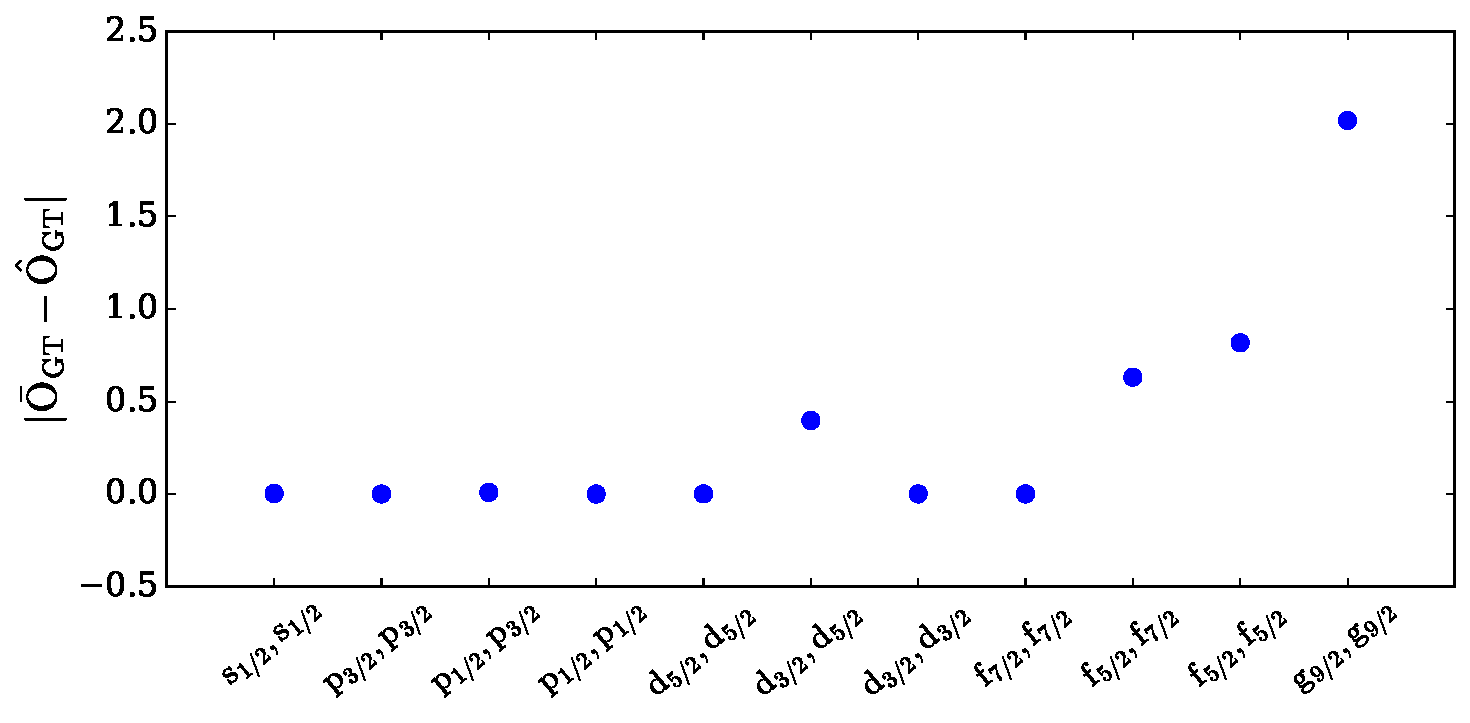
\includegraphics[width=\textwidth]{EOM/BetaMEs.pdf}
  \caption{Difference between bare and similarity transformed Gamow-Teller matrix elements.}
  \label{fig:GTMEs}
\end{figure}


After constructing the effective operators, the reduced transition amplitudes in Eq.\ \eqref{eq:RTAmps} can be calculated.  Because of the ambiguity in the bi-orthonormalization discussed in section \ref{section:eom_dual}, the square-norm of the matrix elements, $\lvert M \rvert^{2}$, must be written using both the left and right solutions for each of the initial and final states.  Expanded in terms of the EOM states, these reduced amplitudes for the Fermi and Gamow-Teller operators become,
\begin{gather}
  B_{F} = \frac{g_{V}^{2}}{2J_{i} + 1}\delta_{J_\mathrm{f}J_{\mathrm{i}}}\sum_{pq}\relement{\Ref}{\Lop_{\mathrm{i}}\EOop{}_{F^{\pm}}\Rop_{\mathrm{f}}}{\Ref}\relement{\Ref}{\Lop_{\mathrm{f}}\EOop{}_{F^{\mp}}\Rop_{\mathrm{i}}}{\Ref}, \\
  B_{GT} = \frac{g_{A}^{2}}{2J_{i} + 1}\sum_{pq}\relement{\Ref}{\Lop_{\mathrm{i}}\EOop{}_{GT^{\pm}}\Rop_{\mathrm{f}}}{\Ref}\relement{\Ref}{\Lop_{\mathrm{f}}\EOop{}_{GT^{\mp}}\Rop_{\mathrm{i}}}{\Ref}.
\end{gather}

Using the machinery developed in this thesis and the techniques discussed in this chapter, the calculated half-lives of various nuclei will be presented in an upcoming paper.


\end{document}
